% Created with Brian Amberg's LaTeX Poster Template. Please refer for the     %
% attached README.md file for the details how to compile with `pdflatex`.     %
% --------------------------------------------------------------------------- %
% $LastChangedDate:: 2011-09-11 10:57:12 +0200 (V, 11 szept. 2011)          $ %
% $LastChangedRevision:: 128                                                $ %
% $LastChangedBy:: rlegendi                                                 $ %
% $Id:: poster.tex 128 2011-09-11 08:57:12Z rlegendi                        $ %
% --------------------------------------------------------------------------- %
\documentclass[a0paper,portrait]{baposter}

\usepackage{relsize}		% For \smaller
\usepackage{url}			% For \url
\usepackage{epstopdf}	% Included EPS files automatically converted to PDF to include with pdflatex
\usepackage{moresize}
\usepackage{multicol}
\usepackage[font=small,labelfont=bf]{subcaption} % <-- changed to subcaption
\usepackage{natbib}

\renewcommand{\bibsection}{}


%%% Global Settings %%%%%%%%%%%%%%%%%%%%%%%%%%%%%%%%%%%%%%%%%%%%%%%%%%%%%%%%%%%

\graphicspath{{pix/}}	% Root directory of the pictures 
\tracingstats=2			% Enabled LaTeX logging with conditionals

%%% Color Definitions %%%%%%%%%%%%%%%%%%%%%%%%%%%%%%%%%%%%%%%%%%%%%%%%%%%%%%%%%

\definecolor{bordercol}{RGB}{40,40,40}
\definecolor{headercol1}{HTML}{DEEEB2}
\definecolor{headercol2}{RGB}{80,80,80}
\definecolor{headerfontcol}{RGB}{0,0,0}
\definecolor{boxcolor}{HTML}{ffffff}

%\definecolor{orange}{HTML}{FF7F00}

%%%%%%%%%%%%%%%%%%%%%%%%%%%%%%%%%%%%%%%%%%%%%%%%%%%%%%%%%%%%%%%%%%%%%%%%%%%%%%%%
%%% Utility functions %%%%%%%%%%%%%%%%%%%%%%%%%%%%%%%%%%%%%%%%%%%%%%%%%%%%%%%%%%

%%% Save space in lists. Use this after the opening of the list %%%%%%%%%%%%%%%%
\newcommand{\compresslist}{
	\setlength{\itemsep}{1pt}
	\setlength{\parskip}{0pt}
	\setlength{\parsep}{0pt}
}

%%%%%%%%%%%%%%%%%%%%%%%%%%%%%%%%%%%%%%%%%%%%%%%%%%%%%%%%%%%%%%%%%%%%%%%%%%%%%%%
%%% Document Start %%%%%%%%%%%%%%%%%%%%%%%%%%%%%%%%%%%%%%%%%%%%%%%%%%%%%%%%%%%%
%%%%%%%%%%%%%%%%%%%%%%%%%%%%%%%%%%%%%%%%%%%%%%%%%%%%%%%%%%%%%%%%%%%%%%%%%%%%%%%

\begin{document}
	\hyphenation{systematic}
\typeout{Poster rendering started}

%%% Setting Background Image %%%%%%%%%%%%%%%%%%%%%%%%%%%%%%%%%%%%%%%%%%%%%%%%%%
\background{
%	\begin{tikzpicture}[remember picture,overlay]%
%	\draw (current page.north west)+(-2em,2em) node[anchor=north west]
%	{\includegraphics[height=1.1\textheight]{background}};
%	\end{tikzpicture}
}

%%% General Poster Settings %%%%%%%%%%%%%%%%%%%%%%%%%%%%%%%%%%%%%%%%%%%%%%%%%%%
%%%%%% Eye Catcher, Title, Authors and University Images %%%%%%%%%%%%%%%%%%%%%%
\begin{poster}{
%	grid=false,
	columns=3,
	colspacing=4.2mm,
	headerheight=0.08\textheight,
	background=none,
	eyecatcher=false,
	%posterbox options
	headerborder=closed,
	borderColor=black,
	headershape=rectangle,
	headershade=plain,
	headerColorOne=blue,
	textborder=rectangle,
	boxshade=plain,
	boxColorOne=white,
	headerFontColor=white,
	headerfont=\color{white}\large\bfseries\sffamily,
	textfont=\larger\sffamily,
	linewidth=1pt
}
%%% Eye Cacther %%%%%%%%%%%%%%%%%%%%%%%%%%%%%%%%%%%%%%%%%%%%%%%%%%%%%%%%%%%%%%%
{
	Eye Catcher, empty if option eyecatcher=false - unused
}
%%% Title %%%%%%%%%%%%%%%%%%%%%%%%%%%%%%%%%%%%%%%%%%%%%%%%%%%%%%%%%%%%%%%%%%%%%
{\sf\bf
	\vspace{1em}The safe use of LLMs for screening in systematic reviews
}
%%% Authors %%%%%%%%%%%%%%%%%%%%%%%%%%%%%%%%%%%%%%%%%%%%%%%%%%%%%%%%%%%%%%%%%%%
{
 %\url{https://dx.doi.org/10.1038/s41558-019-0684-5}\\

}
%%% Logo %%%%%%%%%%%%%%%%%%%%%%%%%%%%%%%%%%%%%%%%%%%%%%%%%%%%%%%%%%%%%%%%%%%%%%
{
% The logos are compressed a bit into a simple box to make them smaller on the result
\setlength\fboxsep{0pt}
\setlength\fboxrule{0pt}
	\fbox{
		\begin{minipage}[border]{14em}
			\centering
			
\includegraphics[width=6.5em, ]{../pres/images/MCC_Logo_RZ_rgb.jpg}
		\end{minipage}
	}
}



\headerbox{The promise of LLMs}{name=1,column=0,row=0}{

%\includegraphics[width=\linewidth]{../plots/literature_size/pubs_time_wgb_lp.pdf}

LLMs have appeared useful for various tasks, but how can we \textbf{safely} use them to save work while screening?

\medskip

They are temperamental, and they return text, not probabilites
}

\headerbox{Next token probabilities}{name=2,column=0,row=0, below=1}{
	
	%\includegraphics[width=\linewidth]{../plots/literature_size/pubs_time_wgb_lp.pdf}
	
	LLMs are \textbf{probabilistic models}, which calculate the \textbf{probable next token} given a \textbf{prompt}.
	
	\medskip
	
	\cite{wang_zero-shot_2024} showed that we can ask a yes/no question and get a probability-like score by subtracting the probability that the next token is no, from the probability it is yes.
	
	\[
	S(d,t) =
	P(\text{yes}|d,t) - P(\text{no}|d,t)
	\]	
	
	\medskip
	
	But the paper did not contain a way to use these scores to save work in a way that would reliably satisfy our need in systematic reviews for high recall
	
}

\headerbox{Prioritised screening}{name=3,column=0,row=0, below=2}{
	
	%\includegraphics[width=\linewidth]{../plots/literature_size/pubs_time_wgb_lp.pdf}
	
	However, if we have probabistic scores for documents, then we can simply do prioritised screening \textit{with} a reliable \textbf{stopping criteria} \citep{callaghan_statistical_2020}
	\smallskip
	

		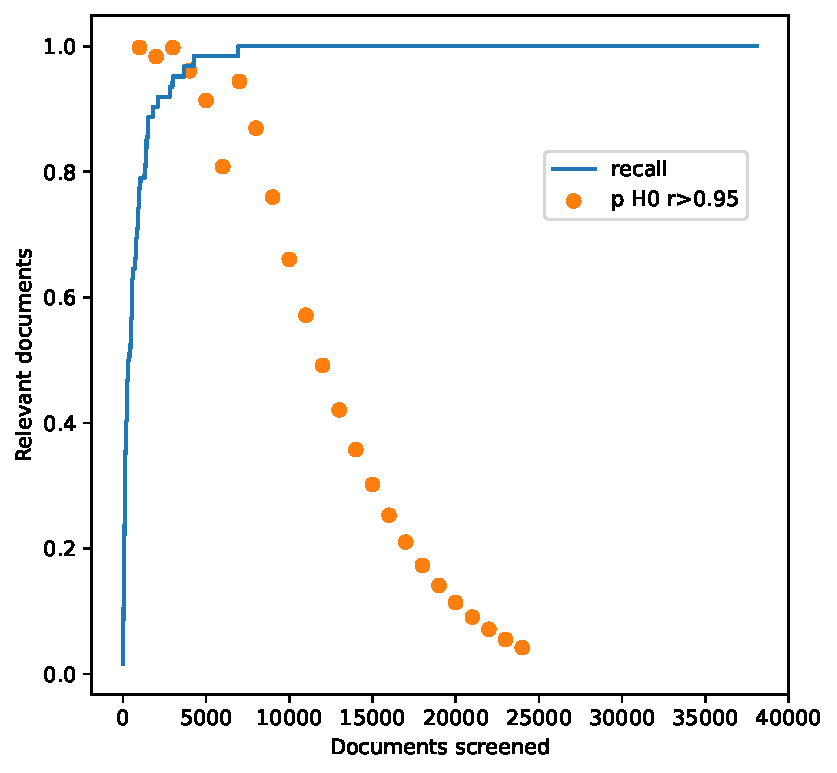
\includegraphics[width=\linewidth]{../../figures/stopping.pdf}

	
}

\headerbox{Results}{name=21,column=1, span=2, row=0}{
	Using the synergy dataset \citep{de_bruin_synergy_2023}, we compared rankings from LLM screening with rankings generated in a traditional ``active learning'' pipeline with SVMs
	
	
	
	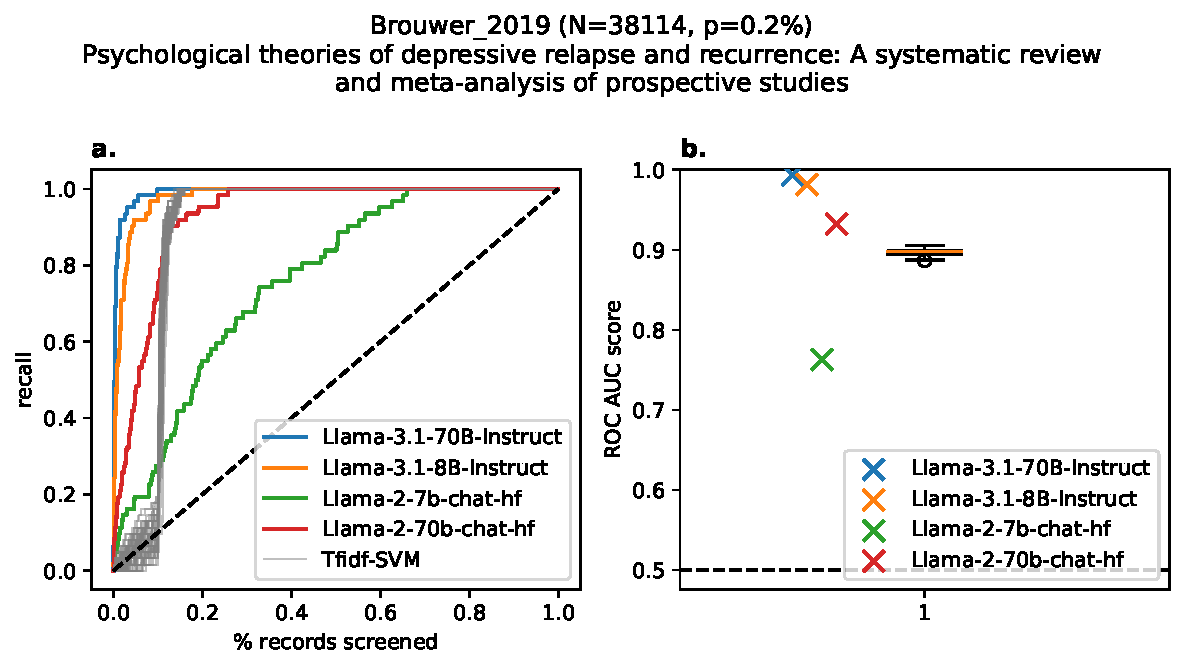
\includegraphics[width=\linewidth]{../../figures/Brouwer_2019.pdf}
	
	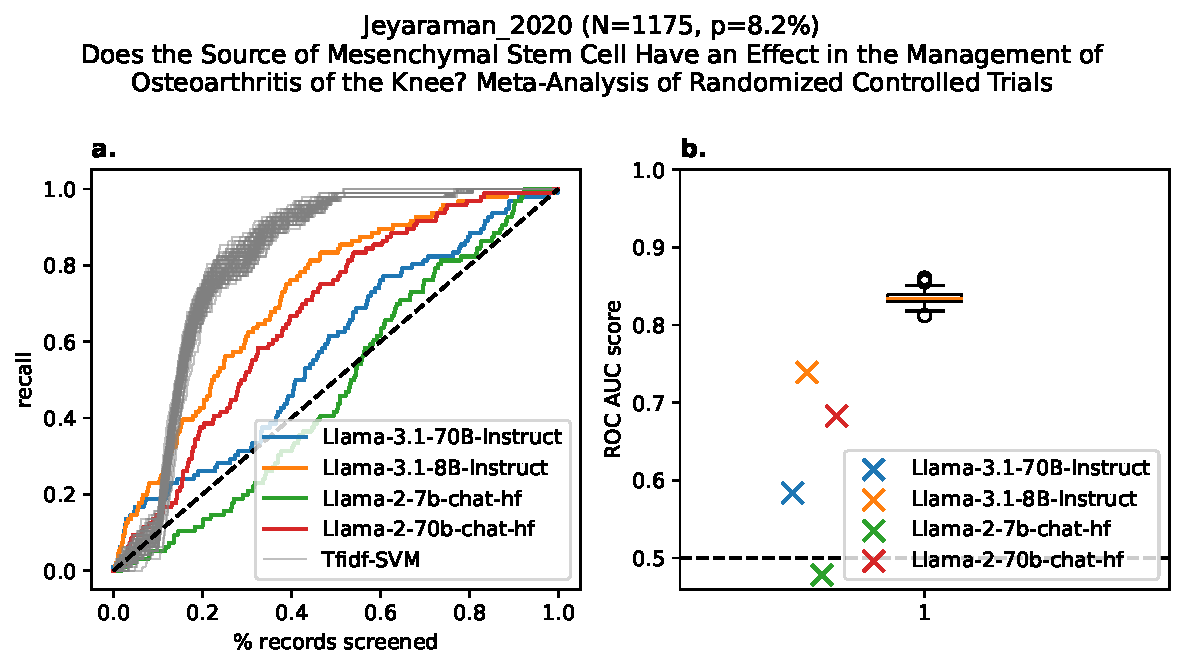
\includegraphics[width=\linewidth]{../../figures/Jeyaraman_2020.pdf}
	
	The best models mostly, but not always, outperform the baseline
}

\headerbox{Results}{name=22,column=1, span=1, below=21}{
	
	
	Llama 3.1 works better than 2 \cite{wang_zero-shot_2024}, and larger models work better than smaller
	
	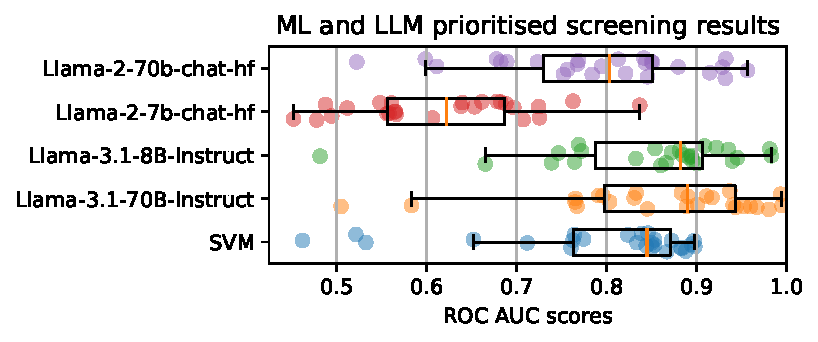
\includegraphics[width=\linewidth]{../../figures/macro_comparison.pdf}

}

\headerbox{Conclusion}{name=32,column=2, span=1, below=21}{
	
	
	Performance with 0 human input is impressive. Combining approaches, or using human labels to provide in-context learning could be promising.
	
}

\headerbox{Bibliography}{name=bib,column=0,row=0, below=3}{
	\scriptsize
	
	%\includegraphics[width=\linewidth]{../plots/literature_size/pubs_time_wgb_lp.pdf}
	\bibliographystyle{apalike}
	\bibliography{../LLMs}
}






\begin{posterbox}[name=footerbox,span=2,column=0,above=bottom,boxheaderheight=0em,textborder=none]{}
{
	For more info on stopping criteria see \url{mcallaghan.github.io/buscar-app} \\
	Max Callaghan \\
{\smaller callaghan@mcc-berlin.net, @MaxCallaghan5}
}
\end{posterbox}








\end{poster}
\end{document}
